%!TEX encoding = IsoLatin

%
% Chapitre "Concept retenu"
%

\chapter{Concept retenu}
\label{s:concept_retenu}

\section{Matrice de décision}

La matrice de décision du projet Fish \& Chips est présentée à la table \ref{t:matrice_decision}. Elle permet d'illustrer clairement le taux de satisfaction de tous les critères pour chaque concept afin de faire un choix éclairé. Les barèmes sont basés sur les critères du tableau \ref{t:criteres} et les pondérations sont ajustées de manière à bien refléter l'importance de chaque besoin du projet. 

\begin{table}[htp]
   \footnotesize
   \centering
   \scalebox{1.0}{
   \begin{tabular}{|c|c||c|c|c|c|}
        \hline
        Critère d'évaluation & Pond. & Concept 1 & Concept 2 & Concept 3 & Concept 4\\
        \hline
        \hline
        \textbf{Qualité du produit} & \textbf{65\%} &\textbf{ \%} &\textbf{ \%} &\textbf{ \%} &\textbf{ \%}\\
        \hline
        Résolution du capteur & 10\% & 8\% & & 3,3 & 2,4 \\
        Identification des poissons & 10\% & 9.1\% & & 9,9 & 10 \\
        Volume d'analyse & 5\% & 1.2\%& & 4,9 & 3,5 \\
        Capacité de stockage des données 
        & 5\% &5\% & & 4 & 5 \\
        Durée de vie de l'alimentation du système & 5\% & 1.3\% & & 3,5 & 3 \\
        Acheminement des informations & 5\% & 4.25\% & & 3,2 & 2\\
        Fiabilité du système de sécurité & 5\% & 4.36\% & & 4,4 &  4,3 \\
        Résistance à la profondeur & 4\% & 0.6\% & & 0,5 & 2\\
        Taille des spécimens observés & 4\% &3.7\% & & & 3,4\\
        Nombre de fonctionnalités de l'alarme & 4\% &0.88\% & & & 0,4\\
        Puissance de calcul & 4\% &3.08\% & & & 1,3 \\
        Utilisation de l'interface graphique & 4\% &4\% & & & 2,4\\
        \hline\hline
        \textbf{Performance} & \textbf{20\%} & \textbf{ \%}  &\textbf{ \%} &\textbf{ \%} &\textbf{ \%} \\
        \hline
        Précision du logiciel de reconnaissance & 15\% &9.1\% & & & 7 \\
        Précision de la régulation & 2\% &2\% & & & 2 \\
        Précision de la mesure de température & 2\% &2\% & & & 1,98 \\
        Précision de la mesure du temps & 1\% &1\% & & & 1 \\
        \hline\hline
        \textbf{Coûts} & \textbf{15\%} &\textbf{ \%} & \textbf{ \%}& \textbf{ \%}&\textbf{ \%} \\
        \hline
        Coût de main d'oeuvre & 12\% & 0\% & & & 9 \\
        Coûts du matériel & 3\% & & & & 3\\
        \hline\hline
        \textbf{Total} & \textbf{100\%} &\textbf{ \%} &\textbf{ \%} &\textbf{ \%} &\textbf{ 63,7\%} \\
        \hline
   \end{tabular}}
    \caption{Matrice de décision du projet Fish \& Chips}
    \label{t:matrice_decision}
\end{table}




\section{Analyse de la matrice de décision}

Avec un taux de satisfaction de xx \%, c'est le concept 2 qui est le mieux adapté aux besoins du projet. Il se démarque surtout par (insérer critère) qui a une plus grande pondération et donc une plus grande importance dans le projet. Les concepts xx, xx et xx ont respectivement des taux de satisfaction de xx\%, xx\% et xx\%. Ils ont surtout des lacunes au niveau de blablabla critères. Le concept 2 est donc retenu et fait l'objet d'une analyse plus détaillée en \ref{ch7:concept_retenu}.

\section{Description du concept retenu}
\label{ch7:concept_retenu}

\textbf{Prise de mesure}
\begin{itemize}
    \item Caméra (OV5640)
    \item Mesure température (thermistance)
    \item Date et heure
\end{itemize}

\textbf{Support physique}
\begin{itemize}
    \item Hardware pour runner le code (PC Custom)
    \item Batterie (rechargeable le best svp)
    \item Régulation (Peltier)
    \item Stockage de données (Carte SD)
    \item Acheminement des infos (Manuel)
\end{itemize}

\textbf{Logique de programmation (renommer)}
\begin{itemize}
    \item Identification (Neurones)
    \item Sécurité (p-e dans comm., encryption?)
\end{itemize}

\textbf{Communication}
\begin{itemize}
    \item Interface graphique (lequel)
    \item Sécurité ??
    \item Envoi de l'alarme (srm Amazon)
\end{itemize}

\clearpage

\subsection{Prise de mesure}

texte de gros requin

\subsection{Support physique}

\subsection{Logique de programmation}

\subsection{Communication}


\section{Conclusion}

lets fucking gooooooooooo

\begin{figure}
    \centering
    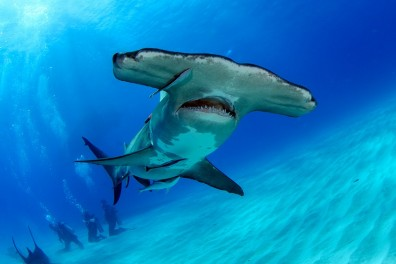
\includegraphics[width=\linewidth]{fig/requinmarto.jpg}
    \caption{Diagramme physique de la solution retenue pour le projet Fish \& Chips}
    \label{fig:concept_retenu}
\end{figure}

